\parindent=0em
\subsection{Asus HC102}
\noindent

Este dispositivo (figura~\ref{fig:asushc102}) apareció en el año 2018 de manos de la empresa Asus, al igual que las \textit{HMD Odyssey+} (punto~\ref{sec:odyssey}), es un dispositivo que requiere ser utilizado junto a un ordenador compatible con \textit{Windows Mixed Reality}, está dotado de sensores para calcular la orientación del usuario como giroscopio, acelerómetro, magnetómetro y sensor de proximidad.\\

\begin{figure}[H]
    \centering
    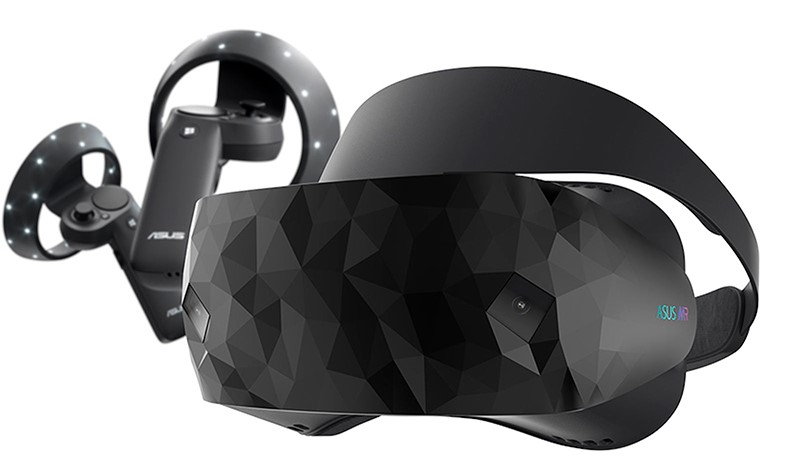
\includegraphics[scale=0.3]{Images/Estado del arte/AsusHC102.jpg}
    \caption[\textit{Asus HC102} al completo]{\textit{Asus HC102} al completo\footnotemark.}
    \label{fig:asushc102}
\end{figure}

\footnotetext{Fuente: \href{https://www.asus.com/Headset/ASUS-Windows-Mixed-Reality-Headset-HC102/specifications/}{\nolinkurl{https://www.asus.com/Headset/ASUSHC102/specifications/}}}

Este casco goza de un FOV de 105\degree , una resolución de 1.440x1.440 por ojo (2.880x1440 en total) y cuenta con dos mandos (cada uno de ellos con un sensor 6DoF) que funcionan con 2 pilas del tipo AA, es decir, 4 pilas AA en total.\\

Finalmente, este HMD permite regular la IPD entre 55mm y 71mm, tiene dos cámaras para hacer un \textit{tracking} de tipo \textit{inside-out} y un peso de 399 gramos.